%%%%%%%%%%%%%%%%%%%%%%%%%%%%%%%%%%%%%%%%%%%%%%%%%%%
%
%  New template code for TAMU Theses and Dissertations starting Fall 2016.
%
%
%  Author: Sean Zachary Roberson 
%	 Version 3.16.09 
%  Last updated 9/12/2016
%
%%%%%%%%%%%%%%%%%%%%%%%%%%%%%%%%%%%%%%%%%%%%%%%%%%%

%%%%%%%%%%%%%%%%%%%%%%%%%%%%%%%%%%%%%%%%%%%%%%%%%%%%%%%%%%%%%%%%%%%%%%
%%                           APPENDIX B
%%%%%%%%%%%%%%%%%%%%%%%%%%%%%%%%%%%%%%%%%%%%%%%%%%%%%%%%%%%%%%%%%%%%%

\chapter{\uppercase {Other Testing}}


\section{SDIRK Convergence Problems}

In order to figure what is causing convergence problems for SDIRK, a manufactured solution was created in the one-dimensional prototype code, described by \eqt{eq:mms}. A second order finite element basis function was used, so the spatial profile was known exactly with only one degree of freedom. The ODE describing this degree of freedom is shown by \eqt{eq:mms_ode}. The coefficients represented in this equation are defined by \eqt{eq:mms_coef}.

\be 
\phi(x,t) = x(1-x)(1+t)^4 \qq 0 \leq x \leq 1
\label{eq:mms}
\ee
\be 
\frac{1}{v}\frac{\partial\phi}{\partial t} = \alpha\phi + \frac{\beta}{v}4(1+t)^3 + \gamma(1+t)^4
\label{eq:mms_ode}
\ee


\begin{subequations}
\be 
\alpha = -D\int_0^1 (4(1-2x))^2dx + (\nu\Sigma_f-\Sigma_a)\int_0^1 (4x(1-x))^2dx = -5.28
\ee
\be 
\beta = \frac{1}{4}\int_0^1(4x(1-x))^2dx = 0.1333
\ee
\be 
\gamma = (\Sigma_a-\nu\Sigma_f)\beta+2D\int_0^1 4x(1-x)dx = 1.32
\ee
\label{eq:mms_coef}
\end{subequations}

The ODE was then evaluated using SDIRK and BDF schemes with varying velocities. \fig{fig:mms1} compares SDIRK and BDF convergence with a relatively large $v$. This plot shows the SDIRK is unable to establish a proper error convergence for such a stiff problem. \fig{fig:mms2} compares SDIRK convergence lines with different velocities. This plot shows that only at relatively small values of $v$, is SDIRK able to show proper convergence.

\begin{figure}[htpb!]
\centering
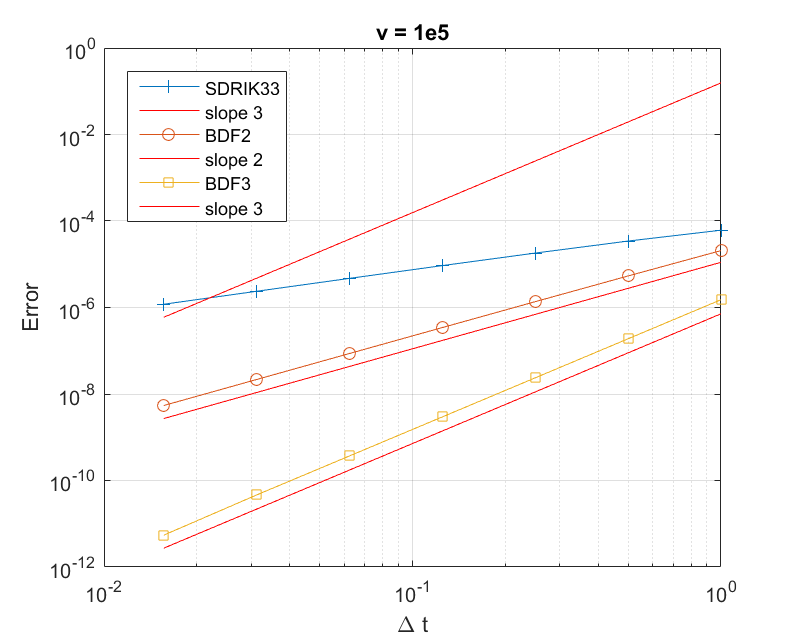
\includegraphics[width=\linewidth]{\FiguresDir/sdirk_mms1.png}
\caption{SDIRK33 vs. BDF convergence with $v=1e5$}
\label{fig:mms1}
\end{figure}

\begin{figure}[htpb!]
\centering
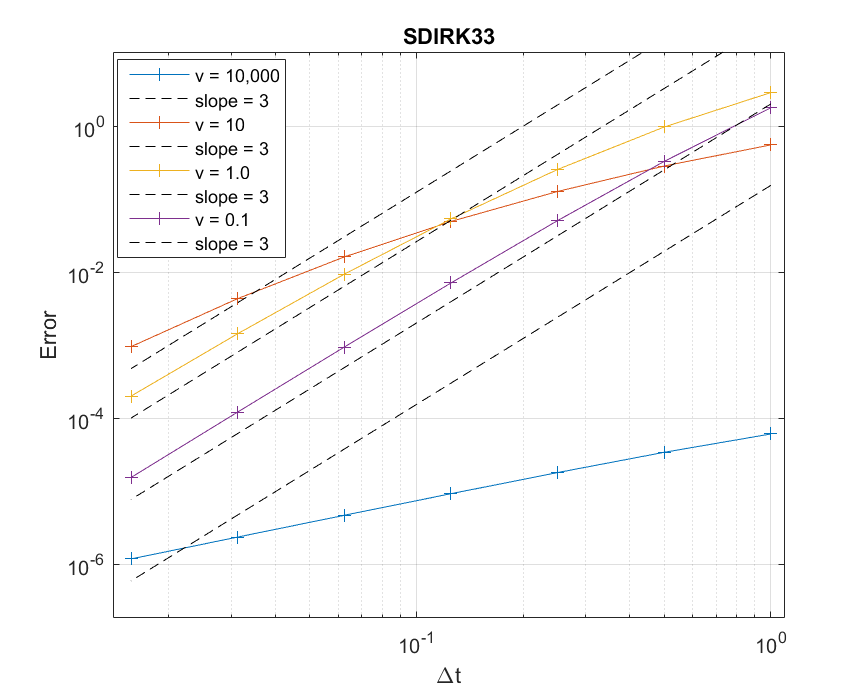
\includegraphics[width=\linewidth]{\FiguresDir/sdirk_mms2.png}
\caption{SDIRK33 convergence with different velocities}
\label{fig:mms2}
\end{figure}

\pagebreak{}